\documentclass{standalone}
\usepackage{amsmath}
\usepackage[usenames,dvipsnames]{xcolor}
\usepackage{tikz}
\usepackage{bm}
\usetikzlibrary{matrix}
\usetikzlibrary{arrows,positioning,decorations.pathreplacing} 

%helvetica
\usepackage[scaled]{helvet}
\renewcommand\familydefault{\sfdefault} 
\usepackage[T1]{fontenc}

\tikzset{
    %Define standard arrow tip
    >=stealth',
    % Define arrow style
    tip/.style={
           ->,
           thin,
           shorten <=2pt,
           shorten >=2pt,}
}

%dotted line stuff
\tikzset{%
  dots/.style args={#1per #2}{%
    line cap=round,
    dash pattern=on 0 off #2/#1
  }
}


\begin{document}


\tikzstyle{full}=[rectangle, draw, 
        minimum width=3cm, minimum
        height=6cm,text width=3cm,
				inner sep=0pt, outer sep=0pt]%
\tikzstyle{tall1}=[rectangle, draw, 
        minimum width=1cm, text centered, minimum
        height=6cm,text width=1cm]%
\tikzstyle{wide1}=[rectangle, draw, 
        minimum width=2.25cm, text centered, minimum
        height=0.8cm,text width=2.25cm]%

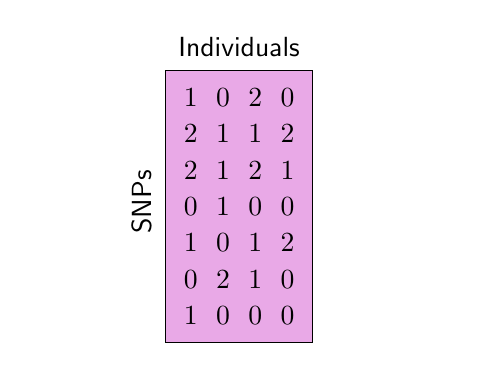
\begin{tikzpicture}[node distance=1cm, auto,]

%start entire figure from Y matrix
\matrix [draw=black,fill=Orchid!60,matrix of math nodes] (Y)
 { 1 & 0 & 2 & 0 \\
  2 & 1 & 1 & 2 \\
  2 & 1 & 2 & 1 \\
  0 & 1 & 0 & 0 \\
	1 & 0 & 1 & 2 \\
	0 & 2 & 1 & 0 \\
	1 & 0 & 0 & 0 \\
};
%label Y
\node[draw=none,fill=none,left=0.05cm of Y](Ytext1){\rotatebox{90}{ SNPs}};
\node[draw=none,fill=none,above=0.05cm of Y](Ytext2){ Individuals};

\node[draw=none,fill=none,right=1.5cm of Y](aa){};
\node[draw=none,fill=none,left=1.5cm of Y](bb){};

\end{tikzpicture}


\end{document} 